\documentclass[journal]{IEEEtran}
\usepackage{cite}
\usepackage{amsmath,amssymb,amsthm}
\usepackage{graphicx}
\usepackage{booktabs}
\usepackage{multirow}
\usepackage{algorithm}
\usepackage{algpseudocode}
\usepackage{url}
\newtheorem{proposition}{Proposition}
\begin{document}
\title{Robust and Privacy-Preserving Federated Intrusion Detection Under Poisoning, Evasion, and Drift in SDN-Enabled IIoT: Extending SFLNID}
\author{First Author, Second Author, and Third Author%
\thanks{Replace with your author and affiliation details.}}
\maketitle

\begin{abstract}
Intrusion detectors trained collaboratively across software-defined industrial IoT networks have to cope with hijacked participants, attackers who adapt, and traffic that keeps changing, yet the recent SFLNID framework leaves all three unresolved. We propose SFLNID-R, which retains the Focal loss, Wasserstein regularization, adaptive differential privacy (DP) and CNN-GRU detector of SFLNID and bolts on three modules. First, Holt--CUSUM Trust Aggregation (HCTA) reuses the Holt forecaster at the server to smooth a median-consensus deviation score, quarantines clients through a CUSUM test, and bounds the influence of the remaining updates. Second, Constraint-Aware Focal Adversarial Training (CAFAT) selects hard attack flows with the Focal factor and perturbs only attacker-controllable features. Third, Drift-Gated Adaptation (DGA) detects drift from a privately released loss signal. We prove a bounded-influence property for HCTA and state how each module changes the DP guarantee. On a synthetic IIoT benchmark that follows the protocol of SFLNID (the original datasets were not reachable), HCTA lowers the backdoor success rate from 0.979 to 0.520 and restores the macro-F1 under a sign-flip attack from 0.051 to 0.732, although it does not outperform Multi-Krum and costs macro-F1 when no attack is present. CAFAT raises the detection of perturbed attacks by 4 to 13 points at a small clean cost. DGA proved unreliable under private release, and we report it as a negative result. We discuss limitations and a path to validation on real data.
\end{abstract}

\begin{IEEEkeywords}
Collaborative learning, industrial IoT, intrusion detection, poisoning robustness, adversarial training, concept drift, differential privacy.
\end{IEEEkeywords}

\section{Introduction}
\IEEEPARstart{N}{etwork} intrusion detection systems (NIDSs) trained with federated learning (FL) have advanced quickly for industrial IoT (IIoT) deployments built on software-defined networking (SDN). Among them, SFLNID~\cite{sflnid} jointly addresses data heterogeneity and privacy leakage by combining a Focal loss with a Wasserstein regularizer, adaptive differential privacy (DP) with Holt-smoothed gradient clipping, and a customized CNN-GRU detector. Its authors, however, explicitly identify three open issues: robustness against \emph{poisoning} of the federated training, robustness against \emph{adversarial} (evasive) traffic, and adaptation to \emph{extreme data drift}. These are not peripheral issues. In SDN-enabled IIoT, the federated clients are domain controllers, i.e., high-value targets that are precisely the nodes an attacker compromises first; the detector is deployed against an adversary that adapts its traffic to the model; and the attack landscape evolves continuously.

Addressing these issues in a framework that already uses DP is harder than in a plain FL setting, for three reasons that we make precise in Section~\ref{sec:design}. First, in SFLNID the clipping and the noise are enforced by the client, so a compromised controller can simply skip them; DP, in this design, is a privacy mechanism, not a robustness mechanism. Second, robust aggregation rules designed for IID data (coordinate-wise median, trimmed mean, Krum)~\cite{krum,yin} discard exactly the signal that non-IID clients legitimately carry, and the interplay of DP and Byzantine robustness is known to be delicate~\cite{zhu_ling}. Third, anomaly-based defenses interpret any change of update behaviour as an attack, so benign concept drift is penalized as misbehaviour~\cite{manias}. Finally, standard adversarial training perturbs all features of a sample, although a network adversary can only manipulate a subset of flow features, and it is blind to the class imbalance that dominates IIoT traffic.

In this paper, we propose \textbf{SFLNID-R}, a robustness extension of SFLNID that leaves the loss design, adaptive DP and CNN-GRU detector of SFLNID as they are and adds three modules, each targeting one open issue:
\begin{enumerate}
\item \textbf{Holt--CUSUM Trust Aggregation (HCTA) against poisoning.} We reuse the Holt level--trend forecaster that SFLNID applies to clipping, but at the server and on a \emph{trust} signal: a median-consensus deviation score is smoothed by Holt, accumulated by a one-sided CUSUM, and a persistently deviating client is quarantined, while the remaining updates are trust-weighted and norm-bounded. HCTA is a post-processing of DP outputs and therefore consumes no privacy budget.
\item \textbf{Constraint-Aware Focal Adversarial Training (CAFAT) against evasion.} The Focal modulating factor of SFLNID is reused as a hardness score to select the attack flows closest to the decision boundary, which are then perturbed by a mimicry PGD restricted to the \emph{attacker-controllable} flow features.
\item \textbf{Drift-Gated Adaptation (DGA) against concept drift.} A Holt forecaster and a CUSUM test run on the log of the privately released, median-aggregated loss that the shared model attains on each client's own data, and they detect drift and trigger a reset of the adaptive clipping states, a short learning-rate boost, and a temporary suspension of quarantine, with the intent that drifted benign clients are not mistaken for attackers (Section~\ref{sec:eval} shows that this intent is not achieved in our current implementation).
\end{enumerate}
The main contributions are as follows.
\begin{itemize}
\item \textbf{Server-Side Holt--CUSUM Trust Aggregation:} We turn the Holt predictor of SFLNID from a client-side clipping heuristic into a server-side temporal trust model. We prove that the influence of any minority of malicious clients is bounded irrespective of their update magnitude, and give the false-quarantine and delay behaviour of the CUSUM detector.
\item \textbf{Feasibility-Constrained, Hardness-Selected Adversarial Training:} CAFAT couples the Focal loss with adversarial training so that imbalance and evasion are handled by one mechanism, and restricts perturbations to the attacker-controllable features.
\item \textbf{Drift Gate and an Honest Negative Result:} We couple a drift detector with the quarantine of the robust aggregator, releasing its signal under the Laplace mechanism. In our experiments this gate is not reliable under private release, and we report why.
\item \textbf{Privacy Accounting and Comprehensive Evaluation:} We state how each module changes the DP guarantee of SFLNID, and evaluate poisoning (two attacks), evasion, drift and their combination, with ablations, detection statistics, and overhead. All experiments use a synthetic benchmark that follows the base protocol, because the original datasets were not reachable.
\end{itemize}

The rest of the article is laid out as follows. Section~II surveys prior work on robust FL, adversarial NIDS and drift, and Section~III widens the threat model. The design of SFLNID-R is given in Section~IV, and Section~V studies its robustness and privacy guarantees. Section~VI reports the experiments, Section~VII covers limitations, and Section~VIII closes the article.

\section{Related Work}
Here we look at prior work on the three open issues of FL-based NIDS: poisoning, evasion, and drift. The base framework SFLNID~\cite{sflnid} and the literature on non-IID FL-based NIDS are not repeated here.

\subsection{Poisoning-Robust Federated Aggregation}
Byzantine-robust aggregators swap the weighted average for statistics that survive when a minority of updates are corrupted. Krum and Multi-Krum keep the updates that sit near their neighbours~\cite{krum}, while the coordinate-wise median and the trimmed mean limit how far extreme coordinates can pull the result~\cite{yin}. Backdoor attacks with model replacement show that a single boosted update can implant a trigger~\cite{bagdasaryan}, and norm clipping of the update has been proposed as a lightweight defense~\cite{sun}. Local model poisoning attacks can be crafted against known aggregation rules~\cite{fang}. All of these assume IID-like benign updates; under non-IID data, the benign spread is large and robust statistics are biased. The relation to DP is also nontrivial: Zhu and Ling show that DP and Byzantine robustness can be bridged through sign-based model-difference aggregation, with privacy and robustness effects that are separate and additive~\cite{zhu_ling}. In contrast to these static, round-wise rules, HCTA keeps a \emph{temporal} model of every client and makes a sequential decision.

\subsection{Adversarial Robustness of Learning-Based NIDS}
Adversarial training with projected gradient descent (PGD) is the standard empirical defense~\cite{madry}. In network traffic, however, features are not freely modifiable: a flow-level adversary can alter packet sizes, timing, and payload lengths, but not the statistics that the defender observes at its own vantage point. Applying unconstrained perturbations over-regularizes the model and, as we show in Section~\ref{sec:eval}, deteriorates the detection of rare attacks. CAFAT restricts the perturbation set to the controllable features and uses the Focal factor to concentrate the training effort on hard attack flows.

\subsection{Concept Drift in Federated Systems}
Concept drift detection in federated networked systems has been addressed by clustering model updates (PCA and K-means) to isolate drifted nodes~\cite{manias}. This is complementary to our goal: rather than identifying which node has drifted, DGA detects \emph{that} a global drift occurred from a privately released loss signal and uses it to protect the learning dynamics (clipping state, learning rate) and the robust aggregator from misinterpreting benign change.

\subsection{Summary}
Existing work treats poisoning, evasion and drift as separate problems and mostly ignores that, in a DP-protected FL-NIDS, they interact: drift is mistaken for poisoning, robust aggregation distorts non-IID learning, and DP noise does not mask poisoned updates. SFLNID-R addresses them jointly while preserving the privacy accounting of SFLNID.

\section{Threat Model}
SFLNID~\cite{sflnid} assumes semi-honest participants and a fixed, stationary attack landscape, and its authors explicitly list poisoning attacks, adversarial evasion and data drift as open issues. We therefore extend the threat model along three axes, while retaining the base assumptions (semi-honest server, DP-protected uploads).
\begin{enumerate}
\item \textbf{Malicious Domain Controllers (Training-Time Poisoning).} Up to $f<K/2$ of the $K$ SDN domain controllers may be compromised. A compromised controller is not bound by the client-side protocol: it may skip the DP noise and the clipping step (which, in SFLNID, are enforced only by the client itself), and it knows the aggregation rule (white-box in the aggregation). We consider two behaviours that start after a warm-up (round $t_a$) so that they appear as a \emph{behavioural change} rather than as a statistical outlier from round one.
\begin{enumerate}
\item \emph{Backdoor with model replacement:} attack flows carrying a trigger pattern in a fixed subset of features are relabeled as \texttt{Normal}, and the resulting update is boosted by a factor $\gamma$~\cite{bagdasaryan}.
\item \emph{Scaled sign-flip:} the honestly computed update is negated and scaled by $\gamma$, an untargeted attack that aims to destroy the global model~\cite{fang}.
\end{enumerate}
\item \textbf{Evasion at Inference Time.} After deployment, the adversary can craft attack traffic whose \emph{controllable} flow features (for instance packet sizes, gaps between packets, payload lengths, flag rates and flow duration) are perturbed within an $\ell_\infty$ budget $\epsilon$ so that the global model classifies it as \texttt{Normal} (mimicry). The remaining features (e.g., aggregate statistics observed at the controller, destination-side counters) cannot be modified without breaking the attack. We evaluate against a white-box PGD adversary~\cite{madry}, i.e., the strongest evaluation attack, restricted to the controllable feature set $\mathcal{C}$.
\item \textbf{Concept Drift.} The attack distribution changes over time (new variants of known attacks). Drift is benign but, from the server's viewpoint, it produces updates that look anomalous, which can trigger false quarantines in any anomaly-based robust aggregator.
\end{enumerate}
Privacy threats are unchanged with respect to~\cite{sflnid}; any new statistic released by our modules is explicitly protected (Section~\ref{sec:priv}).

\section{SFLNID-R Design}\label{sec:design}
This section presents SFLNID-R, which extends SFLNID~\cite{sflnid} with three modules, each targeting one of its open issues: \textbf{A)} Holt--CUSUM Trust Aggregation (HCTA) against poisoning, \textbf{B)} Constraint-Aware Focal Adversarial Training (CAFAT) against evasion, and \textbf{C)} Drift-Gated Adaptation (DGA) against concept drift. We first motivate the design through three observations on SFLNID, then describe the overview and the details of each module. The loss design, adaptive DP and CNN-GRU detector of SFLNID stay exactly as they were.

\subsection{Why SFLNID Needs Server-Side Robustness}
Three properties of the base design motivate our modules. (O1) The adaptive clipping threshold $C_i^t$ of SFLNID is computed and enforced by the client; a compromised controller can ignore it, so the clipping gives \emph{no} protection against poisoning. (O2) The Gaussian noise has standard deviation $\sigma\cdot 2\eta C_i^t/B$ per coordinate, which is tiny compared with a boosted malicious update; DP therefore does not mask poisoning, and it is not a robustness mechanism. (O3) The Holt predictor of SFLNID already encodes a per-client model of ``normal'' behaviour, but it is used only to set $C_i^t$ and is thrown away at the server, while a persistent, predictable deviation is exactly what non-IID benign clients look like. These observations lead us to reuse the Holt forecaster \emph{at the server}, on the \emph{trust} signal, and to combine it with sequential change detection.

\subsection{Overview of SFLNID-R}
Fig.~\ref{fig:overview} shows the extended workflow. On the client side, the SDN domain controller trains with Focal loss, Wasserstein regularization and adaptive DP as in SFLNID, and, if module B is enabled, augments each mini-batch with hard, feasibility-constrained adversarial flows. On the server side, the SDN root controller no longer applies plain FedAvg; the received (already noised) updates pass through HCTA, and the aggregated global loss signal is monitored by DGA, which can reset the adaptive states of both the clients' clipping thresholds and the server's trust states. Because HCTA only post-processes DP outputs and CAFAT only changes the training samples, the DP pipeline of SFLNID is retained (Section~\ref{sec:priv}).

\begin{figure*}[!t]
\centering
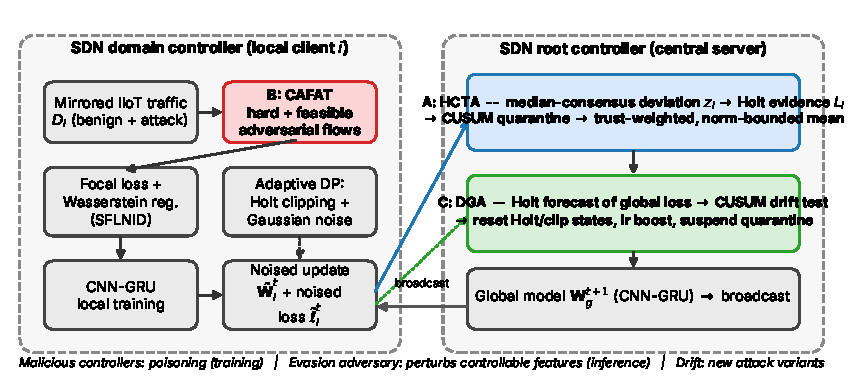
\includegraphics[width=0.85\textwidth]{figs/fig_overview.pdf}
\caption{Overview of SFLNID-R. Modules A, B, and C (highlighted) extend SFLNID on the server side, the client side, and the control loop, respectively.}
\label{fig:overview}
\end{figure*}

\subsection{Module A: Holt--CUSUM Trust Aggregation (HCTA)}
Let $\boldsymbol{\delta}_i^t=\mathbf{W}_i^t-\mathbf{W}_g^t$ be the noised update received from client $i$ in round $t$, $n$ the count of clients taking part, and $\mathbf{m}^t=\mathrm{median}_i(\boldsymbol{\delta}_i^t)$ the coordinate-wise median. HCTA computes, for each client, a \emph{deviation score} that combines a magnitude and a direction term:
\begin{equation}
u_i^t=\frac{\|\boldsymbol{\delta}_i^t-\mathbf{m}^t\|_2}{\mathrm{med}_j\|\boldsymbol{\delta}_j^t-\mathbf{m}^t\|_2}+\Big(1-\cos(\boldsymbol{\delta}_i^t,\mathbf{m}^t)\Big),
\end{equation}
which is standardized across clients with the median and the median absolute deviation (MAD),
\begin{equation}
z_i^t=\frac{u_i^t-\mathrm{med}_j\,u_j^t}{1.4826\,\mathrm{MAD}_j(u_j^t)+\varepsilon_0}.
\end{equation}
The standardization removes the common scale effect of DP noise and learning rate, and the floor $\varepsilon_0$ prevents tiny MAD values from amplifying noise.

\emph{Temporal evidence by Holt smoothing.} A single round is a poor basis for a decision under non-IID data. We therefore smooth the score of every client with the same Holt level--trend recursion that SFLNID uses for clipping, but now applied at the server and on the trust signal:
\begin{align}
H_i^t&=\xi z_i^t+(1-\xi)(H_i^{t-1}+T_i^{t-1}),\\
T_i^t&=\varphi(H_i^t-H_i^{t-1})+(1-\varphi)T_i^{t-1},\\
L_i^t&=H_i^t+\max(0,T_i^t),
\end{align}
where $L_i^t$ is the \emph{evidence} of misbehaviour of client $i$ (the rising-trend term lets the evidence react before the level catches up, and the $\max(\cdot)$ prevents improving clients from being credited twice).

\emph{Sequential decision by CUSUM.} The evidence is accumulated with a one-sided CUSUM statistic~\cite{page},
\begin{equation}
S_i^t=\max\big(0,\,S_i^{t-1}+L_i^t-k\big),\qquad \text{flag}_i^t=\mathbb{1}[S_i^t>h],
\end{equation}
and a flagged client is quarantined (its weight is set to zero); its statistic is decayed, $S_i^t\leftarrow\rho S_i^t$, so that a client that returns to normal behaviour is readmitted (probation). The reference value $k$ absorbs the persistent deviation of benign non-IID clients, and the threshold $h$ trades detection delay against false quarantine (Proposition~\ref{prop:cusum}).

\emph{Trust-weighted, norm-bounded aggregation.} Non-flagged clients receive the soft weight $w_i^t=|D_i|\exp\!\big(-\lambda\max(0,L_i^t-1)\big)$. Finally, every update is bounded by the server, $\hat{\boldsymbol{\delta}}_i^t=\boldsymbol{\delta}_i^t\min\!\big(1,\kappa\tau^t/\|\boldsymbol{\delta}_i^t\|\big)$ with $\tau^t=\mathrm{med}_j\|\boldsymbol{\delta}_j^t\|$, which neutralizes model replacement irrespective of the clipping policy of the client (O1), and
\begin{equation}
\mathbf{W}_g^{t+1}=\mathbf{W}_g^t+\frac{\sum_i w_i^t\,\hat{\boldsymbol{\delta}}_i^t}{\sum_i w_i^t}.
\end{equation}
Algorithm~\ref{alg:hcta} summarizes the procedure. HCTA has $O(nd)$ cost per round (the coordinate-wise median costs $O(nd\log n)$) and needs no server-side data.

\begin{algorithm}[t]
\caption{HCTA: Holt--CUSUM Trust Aggregation}
\label{alg:hcta}
\begin{algorithmic}[1]
\Require Noised updates $\{\boldsymbol{\delta}_i^t\}_{i=1}^n$, sizes $|D_i|$, states $(H_i,T_i,S_i)$, parameters $\xi,\varphi,k,h,\rho,\lambda,\kappa$
\Ensure Global update $\Delta^t$
\State $\mathbf{m}\gets\mathrm{median}_i\,\boldsymbol{\delta}_i$;\ \ $\tau\gets\mathrm{med}_i\|\boldsymbol{\delta}_i\|$
\For{each client $i$}
\State Compute $u_i$ and standardized score $z_i$ \hfill (Eqs.~1--2)
\State Update $H_i,T_i$ and evidence $L_i=H_i+\max(0,T_i)$ \hfill (Eqs.~3--5)
\State $S_i\gets\max(0,S_i+L_i-k)$;\ \ $\text{flag}_i\gets[S_i>h]$
\If{$\text{flag}_i$} $w_i\gets0$;\ $S_i\gets\rho S_i$ \Else\ $w_i\gets|D_i|e^{-\lambda\max(0,L_i-1)}$ \EndIf
\State $\hat{\boldsymbol{\delta}}_i\gets\boldsymbol{\delta}_i\cdot\min(1,\kappa\tau/\|\boldsymbol{\delta}_i\|)$
\EndFor
\State \Return $\Delta^t=\sum_iw_i\hat{\boldsymbol{\delta}}_i/\sum_iw_i$
\end{algorithmic}
\end{algorithm}

\subsection{Module B: Constraint-Aware Focal Adversarial Training (CAFAT)}
Standard adversarial training perturbs all features and all samples, which (i) trains against perturbations that a network attacker cannot realize, (ii) wastes capacity on easy flows, and (iii) conflicts with the class imbalance that SFLNID addresses with the Focal loss. CAFAT instead reuses the Focal modulating factor as a \emph{hardness score} and perturbs only the controllable feature set $\mathcal{C}$.

For a local mini-batch $\mathcal{B}$ and the current local model, let $p_t(x)$ be the probability of the true class. Among the attack samples in $\mathcal{B}$ we select the fraction $\beta$ with the largest hardness $(1-p_t(x))^{\gamma}$ and generate mimicry perturbations with a short, feasibility-constrained PGD:
\begin{equation}
x^{(s+1)}=\Pi_{\|\cdot\|_\infty\le\epsilon_{tr}}\Big(x^{(s)}-\alpha\,\mathrm{sign}\big(\nabla_{x}\mathcal{L}_{CE}(f(x^{(s)}),y_{N})\big)\odot\mathbf{1}_{\mathcal{C}}\Big),
\end{equation}
where $y_N$ is the \texttt{Normal} label, $\mathbf{1}_{\mathcal{C}}$ the indicator of controllable features and $\epsilon_{tr}$ is drawn from $[0.5,1.5]\cdot\epsilon$ per batch to avoid overfitting to one budget. The perturbed samples keep their true (attack) label and are appended to $\mathcal{B}$; the loss of Eq.~(1) of~\cite{sflnid} (Focal loss plus Wasserstein regularization) is then computed on the augmented batch. The cost is $s+1$ additional forward/backward passes on at most $\beta m$ samples ($m$ = number of attack samples in $\mathcal{B}$).

\subsection{Module C: Drift-Gated Adaptation (DGA)}
Concept drift has two harmful side effects in SFLNID-R: the clipping thresholds predicted by the Holt model lag behind the new gradient scale, and drifted benign clients look like outliers to HCTA. DGA spots drift from the global training loss and reacts on both fronts. Each client releases its clipped, Laplace-perturbed mean loss $\tilde\ell_i^t=\min(\ell_i^t,L_{\max})+\mathrm{Lap}\big(L_{\max}/(|D_i|\epsilon_\ell)\big)$ (Section~\ref{sec:priv}); the server forms $\ell^t=\sum_i\tau_i\tilde\ell_i^t$ and applies a Holt forecaster and a CUSUM on its standardized one-step residual:
\begin{equation}
e^t=\ell^t-(H_\ell^{t-1}+T_\ell^{t-1}),\quad z_\ell^t=\frac{e^t}{\hat\sigma_e^t+10^{-3}},\quad G^t=\max(0,G^{t-1}+z_\ell^t-k_\ell),
\end{equation}
where $\hat\sigma_e^2$ is an exponentially weighted estimate of the residual variance. When $G^t>h_\ell$ a drift is declared and DGA (i) resets the Holt states of all clients' clipping predictors and sets each threshold to the largest current threshold, (ii) doubles the learning rate for the next two rounds, and (iii) resets the states of HCTA and suspends quarantine for two rounds, so that drifted benign clients are absorbed rather than excluded.

\section{Theoretical Analysis}
We analyze the influence of malicious clients under HCTA, the false-quarantine and delay behaviour of its CUSUM detector, and the privacy guarantee of SFLNID-R. All statements are conditional on the stated assumptions; the CUSUM statement is an approximation and is validated empirically in Section~\ref{sec:eval}.

\subsection{Robustness Analysis}
\begin{proposition}[Bounded influence]\label{prop:bound}
Denote by $\mathcal{M}$ the malicious clients, with $|\mathcal{M}|<n/2$, and let $\mathcal{B}$ be the benign set. In every round, the contribution of the malicious clients to the aggregated update satisfies
\begin{equation}
\Big\|\frac{\sum_{i\in\mathcal{M}}w_i\hat{\boldsymbol{\delta}}_i}{\sum_{i}w_i}\Big\|_2\le\kappa\max_{j\in\mathcal{B}}\|\boldsymbol{\delta}_j\|_2\cdot\frac{\sum_{i\in\mathcal{M}}w_i}{\sum_iw_i},
\end{equation}
independently of the magnitude of the malicious updates (and hence of the boost factor $\gamma$). In particular, the contribution is zero while the clients in $\mathcal{M}$ are quarantined.
\end{proposition}
\begin{proof}
After the server-side bound, $\|\hat{\boldsymbol{\delta}}_i\|\le\kappa\tau$ with $\tau=\mathrm{med}_j\|\boldsymbol{\delta}_j\|$. Because the adversary owns less than half of the $n$ norms $\|\boldsymbol{\delta}_j\|$, the median falls between the smallest and the largest benign norm, so $\tau\le\max_{j\in\mathcal{B}}\|\boldsymbol{\delta}_j\|$. The triangle inequality over $i\in\mathcal{M}$ gives the claim; $w_i=0$ for quarantined clients.
\end{proof}
Proposition~\ref{prop:bound} explains why scaling attacks (model replacement, scaled sign-flip) are neutralized \emph{even before} the detector fires: the attack is limited to the influence of a normally sized update. It does not bound the \emph{direction} of a stealthy, unboosted update, which is the role of the CUSUM detector.

\begin{proposition}[False quarantine and detection delay, approximate]\label{prop:cusum}
Assume the evidence increments of a benign client are approximately Gaussian with mean $\mu_b<k$ and variance $s^2$, and those of a malicious client have mean $\mu_a>k$. Then (i) the probability that the CUSUM of a benign client ever exceeds $h$ from the zero state is at most $\exp\!\big(-2(k-\mu_b)h/s^2\big)$, and (ii) the expected number of rounds until a malicious client is flagged is approximately $h/(\mu_a-k)$.
\end{proposition}
\begin{proof}[Sketch]
The CUSUM is a random walk with drift $-(k-\mu_b)$ reflected at zero; its supremum is bounded by Lundberg's inequality with adjustment coefficient $\theta^\ast=2(k-\mu_b)/s^2$ for Gaussian increments~\cite{siegmund}. Part~(ii) follows from Wald's identity applied to the first passage time of a random walk with positive drift $\mu_a-k$ across the level $h$~\cite{page,siegmund}. The Holt smoothing makes the increments positively correlated, so the bound should be read as a design guideline (increasing $k$ or $h$ lowers false quarantines and increases delay) rather than as a guarantee.
\end{proof}

\subsection{Privacy Analysis}\label{sec:priv}
\begin{proposition}[Privacy of SFLNID-R]\label{prop:priv}
Let SFLNID satisfy $(T\epsilon,T\delta)$-DP over $T$ rounds (Theorem~5 of~\cite{sflnid}). Then:
(a) HCTA does not consume additional privacy budget;
(b) CAFAT preserves the same guarantee if the Gaussian noise scale is doubled, i.e., $\sigma_{\mathrm{noise}}=2\sigma\cdot2\eta C_i^t/B$;
(c) DGA consumes an additional budget of $T\epsilon_\ell$ for the loss signal (basic composition), independent of the model budget.
\end{proposition}
\begin{proof}
(a) HCTA operates only on the noised uploads $\tilde{\mathbf{W}}_i^t$, which are already $(\epsilon,\delta)$-DP outputs; any function of them is DP by post-processing (Theorem~3 of~\cite{sflnid},~\cite{dwork}). (b) The sensitivity derivation of~\cite{sflnid} bounds the influence of one record by its clipped gradient contribution $2\eta C_i^t/B$. With CAFAT, a record contributes through at most two samples (itself and its adversarial counterpart), so the worst-case sensitivity is at most doubled; the Gaussian mechanism with the same $(\epsilon,\delta)$ then requires doubling the noise scale. (c) The released scalar is bounded by clipping at $L_{\max}$, so its sensitivity is $L_{\max}/|D_i|$ and the Laplace mechanism with scale $L_{\max}/(|D_i|\epsilon_\ell)$ is $\epsilon_\ell$-DP per round, and rounds compose.
\end{proof}
We note that the privacy argument of the base framework treats the per-round sensitivity as in~\cite{sflnid}; Proposition~\ref{prop:priv} inherits this accounting and only states how the new modules change it. In the evaluation we report CAFAT both with unchanged noise and with the privacy-matched doubled noise.

\subsection{Complexity}
HCTA adds $O(nd\log n)$ server computation per round and $O(n)$ state. CAFAT adds $(s+1)$ forward/backward passes on at most $\beta m$ samples per batch on each client. DGA adds $O(1)$ state and one scalar upload per client and round. None of the modules makes the uploaded model any larger, so the communication load is the same as in SFLNID.

\section{Experiments and Results}\label{sec:eval}
\subsection{Experiment Settings}
\textbf{Data and an important caveat.} The datasets that SFLNID relies on (ToN-IoT, RT-IoT and Edge-IIoT) could not be fetched from our environment because the hosting sites were unreachable, so every result below comes from a seeded synthetic IIoT-flow benchmark that mirrors the base protocol: ten traffic classes (one benign class plus nine attack families, among them DDoS, DoS, injection, man-in-the-middle, password, ransomware, scanning and XSS), 19 features, a strongly imbalanced class prior (55\% normal, 1.5\% for \texttt{Mitm}), heavy-tailed class-conditional distributions with overlapping hard classes, and a class-disjoint non-IID split over $K=7$ domain controllers (each controller sees three attack classes plus normal traffic, and every attack class lives on two or three controllers). The first six features are marked attacker-controllable. A centralized CNN-GRU reaches about 0.94 accuracy and 0.93 macro-F1 on this benchmark, and plain non-IID FL about 0.91 and 0.84, so the benchmark is harder than the near-IID numbers reported in the base paper and the absolute values are not comparable with it. The generator, the partition and a loader hook for the real CSV files are in the released code, and the conclusions about real traffic remain to be confirmed.

\textbf{Implementation.} We re-implemented SFLNID (Focal loss, a sorted one-dimensional Wasserstein regularizer, Holt-clipped DP with $(\epsilon,\delta)=(4,10^{-6})$, CNN-GRU with 31,306 parameters) in PyTorch on CPU. Because the original hyperparameters of the clipping multiplier are not given, we use $C_i^t=1.5\,(H_i^t+T_i^t)$ with $\xi=0.99$ and $\varphi=0.01$. We use $K=7$ clients, 16 communication rounds (20 for the drift and combined scenarios), two local epochs, a learning rate of 0.05, momentum of 0.9, mini-batches of 64, $\alpha=0.25$ for the normal class and 0.75 for attack classes, $\gamma=2$, $\lambda=0.1$. Two of seven controllers are malicious from round 4 on (boost $\gamma=4$, backdoor trigger value 4.0 on three non-controllable features, no DP noise from the attacker). \textbf{HCTA} uses $\xi=0.6$, $\varphi=0.2$, $k=1$, $h=3$, $\rho=0.6$, $\lambda=1$, $\kappa=1.5$. \textbf{CAFAT} uses $\beta=0.5$, three PGD steps and $\epsilon=0.5$. \textbf{DGA} uses $\xi=0.9$, $\varphi=0.1$, $k_\ell=0.5$, $h_\ell=3$, a residual scale of 0.1 and a warm-up of four rounds, and releases its signal with $\epsilon_\ell=0.05$ per round. The drift scenario shifts the mean of \texttt{DDoS}, \texttt{DoS} and \texttt{Scanning} at round 10. All hyperparameters of the new modules were chosen on separate tuning seeds (100 and 101); every number below is the mean and standard deviation over seeds 0, 1 and 2, which were not used for tuning. Three seeds give only a coarse estimate of the variance, so small differences should not be over-interpreted.

\textbf{Baselines and metrics.} For poisoning, we compare against FedAvg (the aggregation of SFLNID), coordinate-wise median, trimmed mean, Multi-Krum and server-side norm clipping, all applied on top of the same DP local training. We report accuracy, macro-F1, attack recall (fraction of attack flows classified as any attack), the false-positive rate on normal flows, the backdoor attack success rate (ASR), defined as the share of trigger-carrying attack flows that the model labels \texttt{Normal}, and the detection rate under a white-box 10-step PGD evasion attack on the controllable features with budget $\epsilon$. In our benchmark the trigger alone already moves a share of attack flows to \texttt{Normal} on a clean model, so an ASR of about 0.47 is the floor (the clean FedAvg row).

\subsection{Poisoning Robustness (Module A)}
Table~\ref{tab:agg} and Fig.~\ref{fig:agg} show the results. Without defense, the backdoor attack with model replacement reaches an ASR of 0.979 while keeping macro-F1 at 0.840, i.e., it is invisible in the usual accuracy metrics. The scaled sign-flip attack collapses the FedAvg model (macro-F1 0.051). Coordinate-wise median and trimmed mean do not stop the backdoor (ASR 0.988 and 0.987) and cost a large amount of macro-F1 because they discard the legitimate non-IID signal (0.510 and 0.665 under attack, and 0.427 for the median without any attack). Norm clipping alone leaves an ASR of 0.908. \textbf{HCTA} reduces the ASR to 0.520, close to the floor of 0.471, and restores the macro-F1 under sign-flip from 0.051 to 0.732.

\emph{HCTA does not outperform Multi-Krum.} Multi-Krum reaches a slightly lower ASR (0.481) and higher macro-F1 under both attacks (0.788 versus 0.749 for backdoor, 0.789 versus 0.732 for sign-flip), and the differences are larger than the seed deviation for the sign-flip case. In the attack-free scenario, \textbf{HCTA} keeps a higher macro-F1 than Multi-Krum (0.764 versus 0.715), but it is not free: it loses 7 points of macro-F1 with respect to FedAvg (0.835), because in two of the three clean runs it quarantined one benign client for 7 and 9 rounds. This is the price of a sequential detector with no side information under heterogeneous clients, and we report it as a limitation (Section~VII).

What \textbf{HCTA} offers beyond the aggregate metrics is an explicit, attributable decision. Over all backdoor, sign-flip and clean runs, it flagged 94.2\% of the malicious client-rounds after the attack start, with a mean detection delay of 0.75 rounds (all 12 malicious clients were flagged), and a false-quarantine rate of 3.2\% of benign client-rounds. Fig.~\ref{fig:trust} shows the deviation scores of one run. The server-side time of \textbf{HCTA} is 4.7 ms per round, against 0.6 ms for FedAvg and 3.4 ms for the median, and it does not change the upload size.

\begin{table}[!t]
\centering
\caption{Poisoning Robustness Under DP (Mean $\pm$ Std Over 3 Seeds, 2 of 7 Malicious Clients). In the Attack-Free Block the ASR Column Is the Natural Trigger Rate of a Clean Model.}
\label{tab:agg}
\footnotesize
\renewcommand{\arraystretch}{1.1}
\setlength{\tabcolsep}{3pt}
\resizebox{\ifdim\width>\columnwidth\columnwidth\else\width\fi}{!}{%
\begin{tabular}{lcccc}
\toprule
Method & Accuracy & Macro-F1 & Attack Recall & ASR \\
\midrule
\multicolumn{5}{l}{\textit{No attack}} \\
FedAvg (SFLNID) & 0.907$\pm$.009 & 0.835$\pm$.016 & 0.816$\pm$.025 & 0.471$\pm$.044 \\
Coord.\ Median & 0.723$\pm$.017 & 0.427$\pm$.037 & 0.419$\pm$.035 & 0.839$\pm$.052 \\
Multi-Krum & 0.863$\pm$.028 & 0.715$\pm$.039 & 0.753$\pm$.067 & 0.401$\pm$.068 \\
\textbf{HCTA (ours)} & $\mathbf{0.889\pm.006}$ & $\mathbf{0.764\pm.044}$ & $\mathbf{0.790\pm.002}$ & $\mathbf{0.464\pm.068}$ \\
\multicolumn{5}{l}{\textit{Backdoor + model replacement}} \\
FedAvg (SFLNID) & 0.911$\pm$.009 & 0.840$\pm$.019 & 0.839$\pm$.033 & 0.979$\pm$.010 \\
Coord.\ Median & 0.757$\pm$.025 & 0.510$\pm$.052 & 0.493$\pm$.088 & 0.988$\pm$.015 \\
Trimmed Mean & 0.838$\pm$.006 & 0.665$\pm$.007 & 0.663$\pm$.023 & 0.987$\pm$.008 \\
Multi-Krum & 0.887$\pm$.014 & 0.788$\pm$.003 & 0.782$\pm$.037 & 0.481$\pm$.090 \\
Norm Clipping & 0.893$\pm$.007 & 0.790$\pm$.022 & 0.792$\pm$.018 & 0.908$\pm$.017 \\
\textbf{HCTA (ours)} & $\mathbf{0.878\pm.013}$ & $\mathbf{0.749\pm.044}$ & $\mathbf{0.770\pm.022}$ & $\mathbf{0.520\pm.060}$ \\
\multicolumn{5}{l}{\textit{Scaled sign-flip}} \\
FedAvg (SFLNID) & 0.385$\pm$.230 & 0.051$\pm$.028 & 0.333$\pm$.471 & -- \\
Coord.\ Median & 0.723$\pm$.014 & 0.421$\pm$.012 & 0.466$\pm$.095 & -- \\
Multi-Krum & 0.887$\pm$.012 & 0.789$\pm$.009 & 0.778$\pm$.029 & -- \\
Norm Clipping & 0.791$\pm$.021 & 0.578$\pm$.057 & 0.585$\pm$.046 & -- \\
\textbf{HCTA (ours)} & $\mathbf{0.876\pm.021}$ & $\mathbf{0.732\pm.074}$ & $\mathbf{0.757\pm.046}$ & -- \\

\bottomrule
\end{tabular}}
\end{table}

\begin{figure*}[!t]
\centering
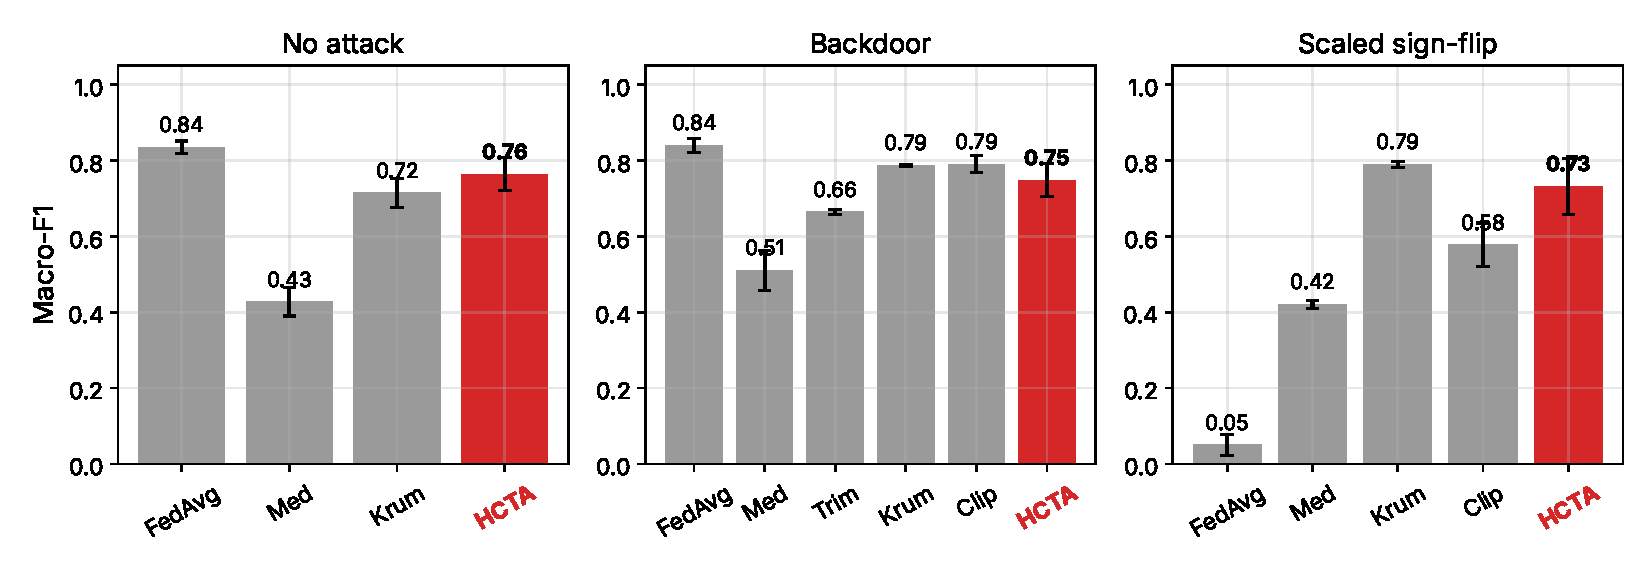
\includegraphics[width=\textwidth]{figs/fig_agg.pdf}
\caption{Macro-F1 of the aggregation rules without attack, under backdoor and under scaled sign-flip (HCTA in red).}
\label{fig:agg}
\end{figure*}

\begin{figure*}[!t]
\centering
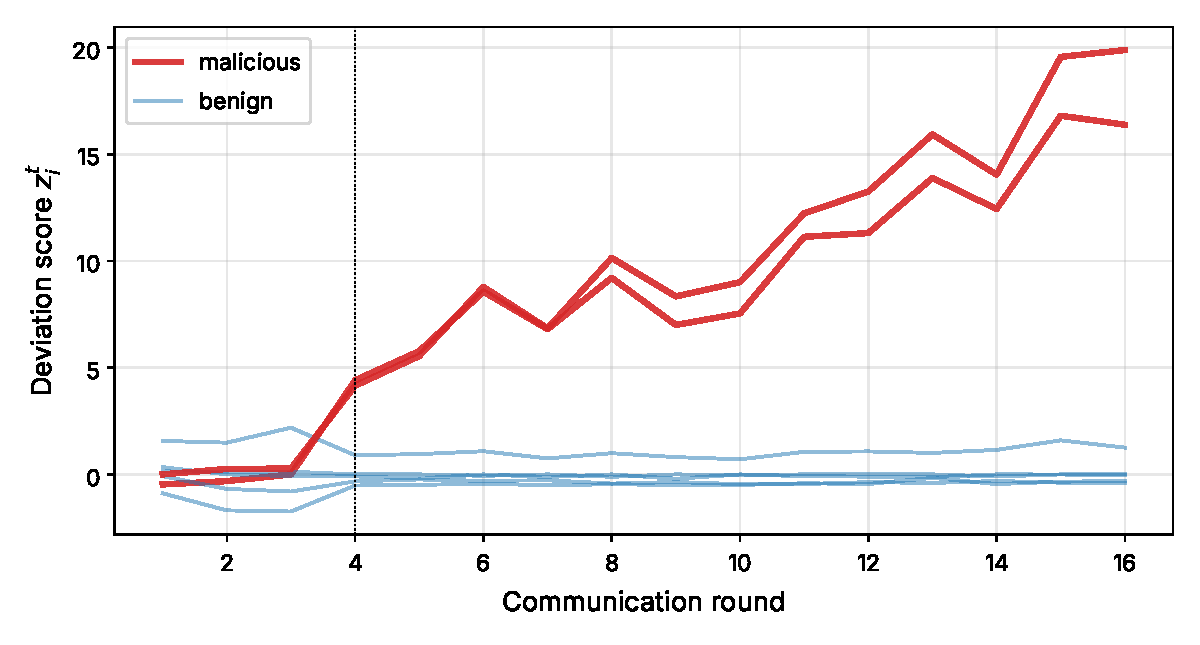
\includegraphics[width=0.62\textwidth]{figs/fig_trust.pdf}
\caption{Deviation scores $z_i^t$ of benign (blue) and malicious (red) clients under the backdoor attack (seed 0). The dotted line marks the first attack round.}
\label{fig:trust}
\end{figure*}

\subsection{Evasion Robustness (Module B)}
Table~\ref{tab:adv} and Fig.~\ref{fig:evasion} report the attack detection rate (the false-positive rates quoted below are from the same runs) when the attacker perturbs the controllable features. The undefended SFLNID model detects 75.2\%, 67.8\% and 51.8\% of the attack flows at $\epsilon=0.25$, 0.5 and 1.0. \textbf{CAFAT} raises these to 79.4\%, 75.0\% and 64.8\% (gains of 4.2, 7.2 and 13.0 points) and changes the clean macro-F1 only from 0.835 to 0.829. Naive PGD adversarial training, which perturbs all features of all attack samples, gives similar detection rates (79.4\%, 75.6\%, 67.2\%), so on robustness alone \textbf{CAFAT} is \emph{not} better than the naive variant. The difference is the price paid on clean traffic: naive training lowers the macro-F1 to 0.801 and doubles the false-positive rate with respect to the baseline (0.016 versus 0.007), while \textbf{CAFAT} stays at 0.012. Following Proposition~\ref{prop:priv}, we also trained \textbf{CAFAT} with doubled noise so that the $(\epsilon,\delta)$ guarantee is preserved under the worst-case doubled sensitivity: the detection rates (80.1\%, 75.7\%, 66.2\%) and the macro-F1 (0.837) are indistinguishable from the unchanged-noise version, so this privacy correction is free in practice. The cost of \textbf{CAFAT} is client-side computation: a communication round takes 10.6 s against 5.3 s for the baseline (about 2.0 times) in our CPU implementation.

\begin{table}[!t]
\centering
\caption{Attack Detection Rate Under White-Box PGD Evasion of Controllable Features, and Clean Macro-F1 (3 Seeds).}
\label{tab:adv}
\footnotesize
\renewcommand{\arraystretch}{1.1}
\setlength{\tabcolsep}{3pt}
\resizebox{\ifdim\width>\columnwidth\columnwidth\else\width\fi}{!}{%
\begin{tabular}{lccccc}
\toprule
Method & $\epsilon$=0 & 0.25 & 0.5 & 1.0 & F1 \\
\midrule
SFLNID & 0.816$\pm$.025 & 0.752$\pm$.027 & 0.678$\pm$.027 & 0.518$\pm$.026 & 0.835$\pm$.016 \\
Naive PGD-AT & 0.824$\pm$.010 & 0.794$\pm$.011 & 0.756$\pm$.009 & 0.672$\pm$.006 & 0.801$\pm$.006 \\
\textbf{CAFAT} & $\mathbf{0.832\pm.013}$ & $\mathbf{0.794\pm.017}$ & $\mathbf{0.750\pm.018}$ & $\mathbf{0.648\pm.017}$ & $\mathbf{0.829\pm.011}$ \\
\textbf{CAFAT (DP-matched)} & $\mathbf{0.841\pm.013}$ & $\mathbf{0.801\pm.015}$ & $\mathbf{0.757\pm.017}$ & $\mathbf{0.662\pm.013}$ & $\mathbf{0.837\pm.018}$ \\

\bottomrule
\end{tabular}}
\end{table}

\begin{figure*}[!t]
\centering
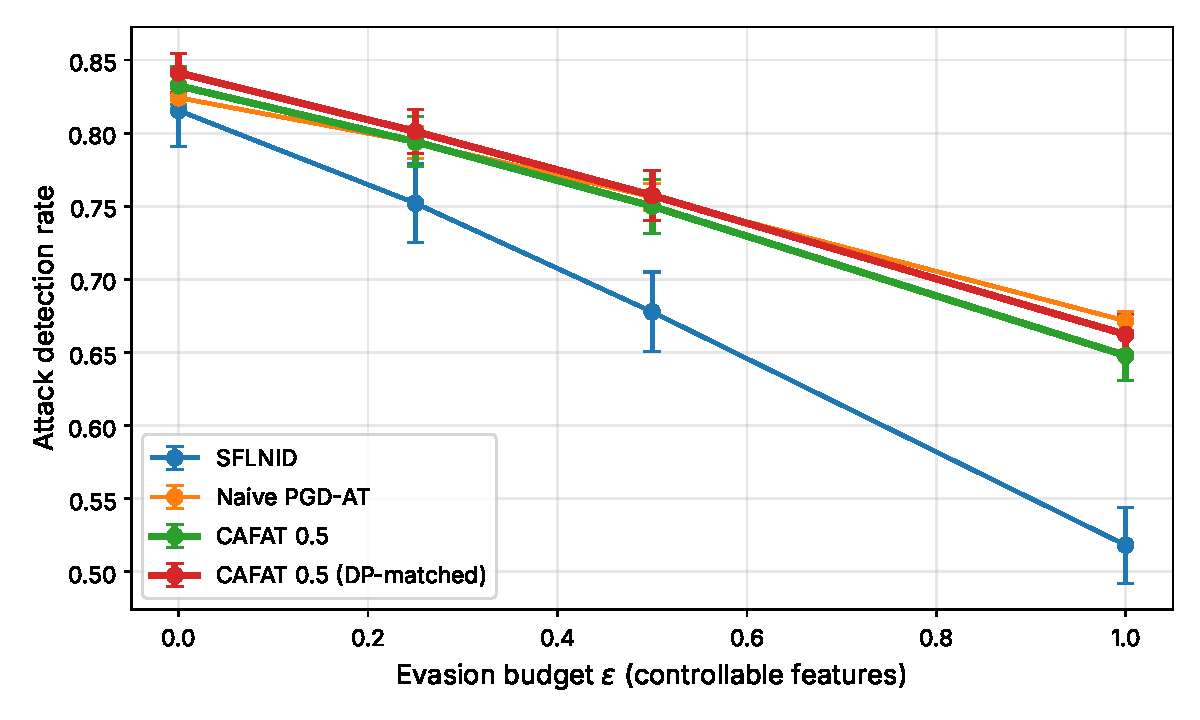
\includegraphics[width=0.62\textwidth]{figs/fig_evasion.pdf}
\caption{Attack detection rate versus evasion budget.}
\label{fig:evasion}
\end{figure*}

\subsection{Drift-Gated Adaptation (Module C): A Negative Result}
Table~\ref{tab:drift} and Fig.~\ref{fig:drift} show that \textbf{DGA}, in its current form, does not help. After the drift at round 10, the lowest post-drift macro-F1 of SFLNID is 0.706 and that of SFLNID with \textbf{DGA} is 0.683, and the final macro-F1 is 0.859 and 0.845. With \textbf{HCTA}, the gate does not repair the quarantine problem either (final 0.791 without and 0.815 with the gate, a difference within the seed spread of 0.039). The reason is the detector. In the drift runs it fired within one round of the drift in two of three seeds (rounds 10 and 11) but also raised two to three additional alarms per run, and in the control experiment without any drift it still fired two or three times in all three seeds (macro-F1 0.853, 0.769 and 0.871 against 0.846, 0.839 and 0.862 without gate). We tuned the detector offline on noise-free probe losses of the tuning seeds and then ran it with the Laplace noise needed for privacy, whose relative magnitude grows as the loss decays; we believe this mismatch explains the false alarms, but we did not verify this. Each false alarm resets the clipping state and, when \textbf{HCTA} is active, suspends quarantine for two rounds, which is why adding \textbf{DGA} to \textbf{HCTA} raises the backdoor ASR in the combined scenario below. The drift in our benchmark is also mild: at round 10 the macro-F1 of SFLNID is 0.706 with the drift and 0.736 in the control without drift, and the gap has closed by round 14 (0.798 against 0.800), so there is little room for any gate to help.

\begin{table}[!t]
\centering
\caption{Drift at Round 10 (No Attack): Macro-F1 at Round 9 (Pre), Lowest Macro-F1 After the Drift, Mean Macro-F1 After the Drift, and Final Macro-F1.}
\label{tab:drift}
\footnotesize
\renewcommand{\arraystretch}{1.1}
\setlength{\tabcolsep}{3pt}
\resizebox{\ifdim\width>\columnwidth\columnwidth\else\width\fi}{!}{%
\begin{tabular}{lcccc}
\toprule
Method & Pre F1 & Min F1 & Mean F1 & Final F1 \\
\midrule
SFLNID & $0.706\pm.029$ & $0.706\pm.008$ & $0.800\pm.005$ & $0.859\pm.018$ \\
\textbf{SFLNID + C} & $\mathbf{0.706\pm.029}$ & $\mathbf{0.683\pm.014}$ & $\mathbf{0.776\pm.008}$ & $\mathbf{0.845\pm.026}$ \\
\textbf{SFLNID + A} & $\mathbf{0.671\pm.056}$ & $\mathbf{0.663\pm.031}$ & $\mathbf{0.745\pm.037}$ & $\mathbf{0.791\pm.039}$ \\
\textbf{SFLNID + A + C} & $\mathbf{0.671\pm.056}$ & $\mathbf{0.652\pm.017}$ & $\mathbf{0.742\pm.019}$ & $\mathbf{0.815\pm.012}$ \\

\bottomrule
\end{tabular}}
\end{table}

\begin{figure*}[!t]
\centering
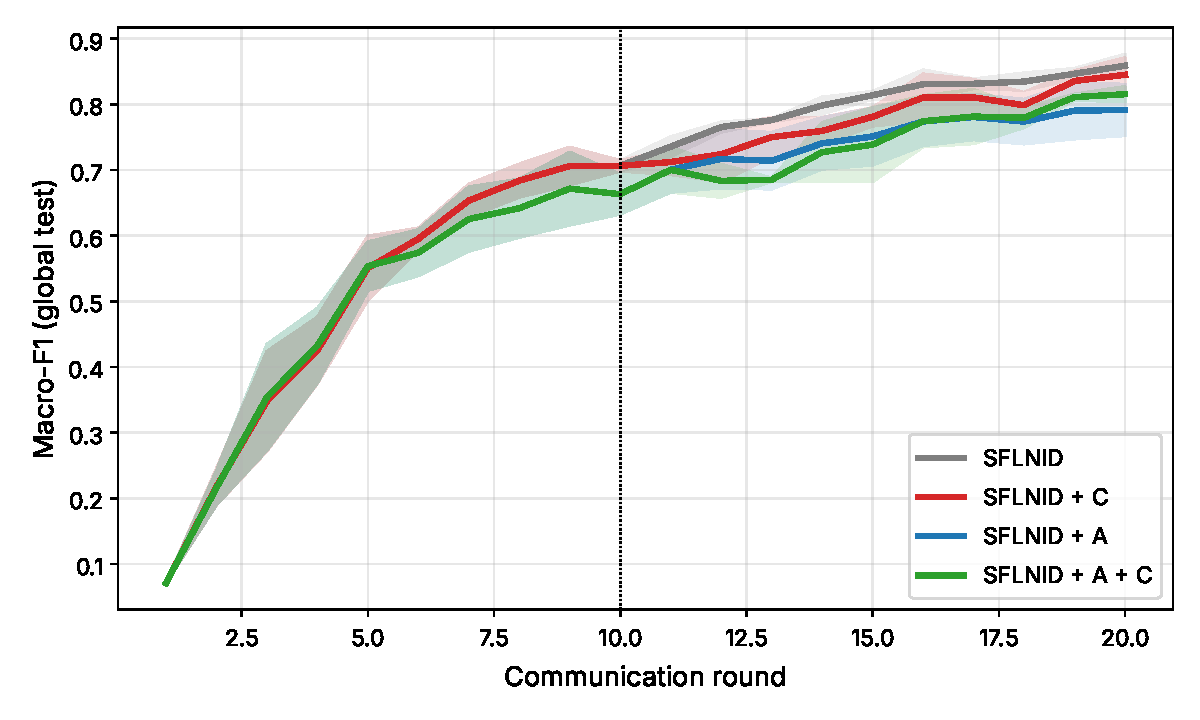
\includegraphics[width=0.62\textwidth]{figs/fig_drift.pdf}
\caption{Macro-F1 around the drift (round 10).}
\label{fig:drift}
\end{figure*}

\subsection{Combined Scenario and Ablation}
Table~\ref{tab:abl} and Fig.~\ref{fig:abl} combine a backdoor attack with the drift of round 10 and evaluate all module combinations. The base model has an ASR of 0.970 and detects 71.7\% of the attacks at $\epsilon=0.5$. \textbf{HCTA} alone lowers the ASR to 0.331 but costs macro-F1 (0.750 against 0.855, with a large spread of 0.068). \textbf{CAFAT} alone improves the detection at $\epsilon=0.5$ to 0.781 and, surprisingly, also lowers the ASR slightly (0.893); we did not investigate why. The combination \textbf{HCTA}+\textbf{CAFAT} (A+B) is the best configuration in this study for the joint threat: ASR 0.323, detection 0.755 at $\epsilon=0.5$, macro-F1 0.805. The full model with \textbf{DGA} is worse than A+B on the ASR (0.712), because the gate fires several times per run and each firing suspends quarantine. We therefore recommend A+B and do not recommend module C in its present form.

\begin{table}[!t]
\centering
\caption{Ablation Under Backdoor Attack and Drift at Round 10 (3 Seeds). Detection Is Measured at $\epsilon=0.5$.}
\label{tab:abl}
\footnotesize
\renewcommand{\arraystretch}{1.1}
\setlength{\tabcolsep}{3pt}
\resizebox{\ifdim\width>\columnwidth\columnwidth\else\width\fi}{!}{%
\begin{tabular}{lcccccc}
\toprule
Config. & A & B & C & F1 & ASR & Det. \\
\midrule
SFLNID &  &  &  & 0.855$\pm$.009 & 0.970$\pm$.009 & 0.717$\pm$.017 \\
\textbf{+A} & \checkmark &  &  & $\mathbf{0.750\pm.068}$ & $\mathbf{0.331\pm.045}$ & $\mathbf{0.690\pm.021}$ \\
\textbf{+B} &  & \checkmark &  & $\mathbf{0.867\pm.020}$ & $\mathbf{0.893\pm.024}$ & $\mathbf{0.781\pm.040}$ \\
\textbf{+C} &  &  & \checkmark & $\mathbf{0.830\pm.038}$ & $\mathbf{0.973\pm.001}$ & $\mathbf{0.675\pm.072}$ \\
\textbf{+A+B} & \checkmark & \checkmark &  & $\mathbf{0.805\pm.009}$ & $\mathbf{0.323\pm.053}$ & $\mathbf{0.755\pm.014}$ \\
\textbf{+A+C} & \checkmark &  & \checkmark & $\mathbf{0.786\pm.035}$ & $\mathbf{0.622\pm.092}$ & $\mathbf{0.710\pm.014}$ \\
\textbf{SFLNID-R} & \checkmark & \checkmark & \checkmark & $\mathbf{0.810\pm.041}$ & $\mathbf{0.712\pm.053}$ & $\mathbf{0.741\pm.054}$ \\

\bottomrule
\end{tabular}}
\end{table}

\begin{figure*}[!t]
\centering
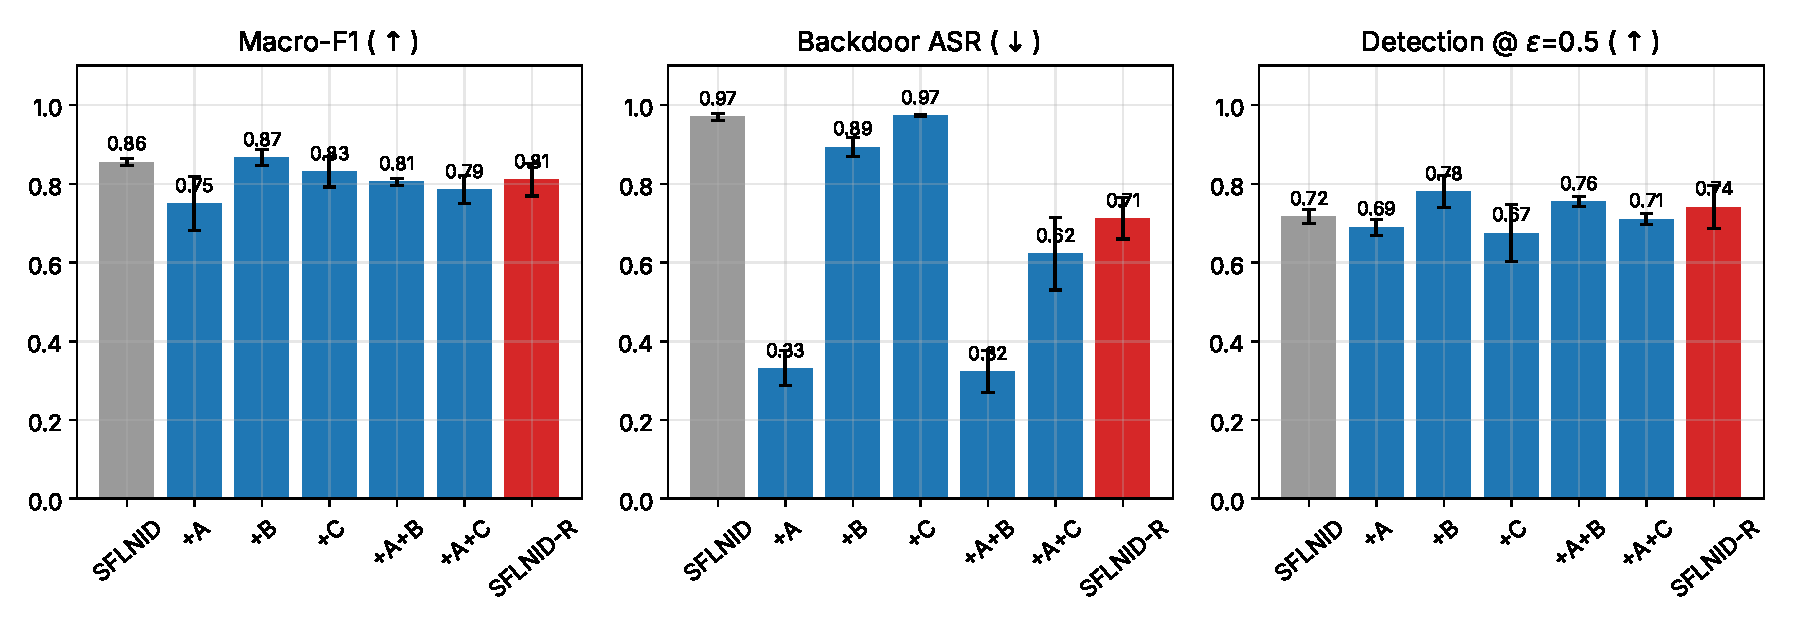
\includegraphics[width=\textwidth]{figs/fig_abl.pdf}
\caption{Ablation of the modules in the combined scenario (full model in red).}
\label{fig:abl}
\end{figure*}

\subsection{Privacy and Overhead}
\textbf{HCTA} is applied to already noised updates and consumes no budget. \textbf{CAFAT} keeps $(\epsilon,\delta)$ when the noise is doubled, with no measurable utility change (above). \textbf{DGA} releases a scalar per client and round with $\epsilon_\ell=0.05$, which composes to 1.0 over the 20 rounds of the drift scenario, in addition to the model budget. The upload size is unchanged (31,306 parameters). Client computation doubles with \textbf{CAFAT}, and the server cost of \textbf{HCTA} is a few milliseconds per round.

\section{Limitation Discussion}
Our study has several limitations. First, and most important, the experiments use a synthetic benchmark that mimics the protocol of the base paper; we could not obtain the real ToN-IoT, RT-IoT and Edge-IIoT data, and the assignment of the real features to the controllable subset has to be defined by domain experts. Second, \textbf{HCTA} does not beat Multi-Krum, and it quarantined a benign client in two of three clean runs; the benefit of quarantine is attribution, not accuracy, and quarantine always costs the data of the excluded client. Our tuning on a small partition of the seeds showed that giving flagged clients partial weight or clipping them to the benign coordinate envelope recovers at most 0.02 macro-F1 and lets the backdoor survive (ASR 0.62 to 0.97), so a better way to keep the benign knowledge of a compromised client is still missing. Third, \textbf{CAFAT} matches naive adversarial training on robustness and its advantage is limited to the clean-traffic cost; it was evaluated only against a PGD mimicry attack. Fourth, the drift gate failed to be reliable under private release; it was tuned on noise-free signals and we did not tune it under noise. Fifth, only two attack types, one malicious fraction (2 of 7), and three seeds were evaluated, adaptive attacks against \textbf{HCTA} (for example slow-drifting poisoning) were not tested, and the DP accounting inherits the sensitivity analysis of the base paper. Future work will replace the synthetic data with the real datasets, make the drift detector noise-aware, and study adaptive and slow poisoning.

\section{Conclusion}
In this article, we extended SFLNID with modules aimed at its stated open issues: poisoning, adversarial evasion, and drift. On a synthetic benchmark that follows the base protocol, Holt--CUSUM trust aggregation neutralized a boosted backdoor (ASR from 0.979 to 0.520) and a scaled sign-flip attack (macro-F1 from 0.051 to 0.732) with an attributable decision, but did not outperform Multi-Krum and had a clean-data cost. Constraint-aware focal adversarial training improved the detection of perturbed attacks by 4 to 13 points at a small clean cost, and its privacy-matched version came for free. The drift-gated adaptation did not work reliably and we report it as a negative result. The best configuration for the joint threat was the combination of the first two modules. Confirmation on real IIoT datasets is the immediate next step.

\begin{thebibliography}{99}
\bibitem{sflnid} T.~Hu, Q.~Chen, Y.~Hu, S.~Hou, H.~Yan, P.~Yi, and Z.~Cui, ``Efficient and privacy-preserving network intrusion detection based on federated learning in SDN-enabled IIoT network,'' \emph{IEEE Internet Things J.}, 2025, doi: 10.1109/JIOT.2025.3591598.
\bibitem{fedavg} B.~McMahan, E.~Moore, D.~Ramage, S.~Hampson, and B.~A.~y~Arcas, ``Communication-efficient learning of deep networks from decentralized data,'' in \emph{Proc. 20th Int. Conf. Artif. Intell. Statist.}, 2017, pp. 1273--1282.
\bibitem{krum} P.~Blanchard, E.~M.~El~Mhamdi, R.~Guerraoui, and J.~Stainer, ``Machine learning with adversaries: Byzantine tolerant gradient descent,'' in \emph{Proc. Adv. Neural Inf. Process. Syst.}, 2017, pp. 119--129.
\bibitem{yin} D.~Yin, Y.~Chen, K.~Ramchandran, and P.~Bartlett, ``Byzantine-robust distributed learning: Towards optimal statistical rates,'' in \emph{Proc. 35th Int. Conf. Mach. Learn.}, 2018, pp. 5650--5659.
\bibitem{sun} Z.~Sun, P.~Kairouz, A.~T.~Suresh, and H.~B.~McMahan, ``Can you really backdoor federated learning?'' \emph{arXiv:1911.07963}, 2019.
\bibitem{bagdasaryan} E.~Bagdasaryan, A.~Veit, Y.~Hua, D.~Estrin, and V.~Shmatikov, ``How to backdoor federated learning,'' in \emph{Proc. 23rd Int. Conf. Artif. Intell. Statist.}, 2020, pp. 2938--2948.
\bibitem{fang} M.~Fang, X.~Cao, J.~Jia, and N.~Gong, ``Local model poisoning attacks to Byzantine-robust federated learning,'' in \emph{Proc. 29th USENIX Security Symp.}, 2020, pp. 1605--1622.
\bibitem{zhu_ling} H.~Zhu and Q.~Ling, ``Bridging differential privacy and Byzantine-robustness via model aggregation,'' in \emph{Proc. 31st Int. Joint Conf. Artif. Intell.}, 2022 (arXiv:2205.00107).
\bibitem{madry} A.~Madry, A.~Makelov, L.~Schmidt, D.~Tsipras, and A.~Vladu, ``Towards deep learning models resistant to adversarial attacks,'' in \emph{Proc. Int. Conf. Learn. Represent.}, 2018.
\bibitem{manias} D.~M.~Manias, I.~Shaer, L.~Yang, and A.~Shami, ``Concept drift detection in federated networked systems,'' \emph{arXiv:2109.06088}, 2021.
\bibitem{page} E.~S.~Page, ``Continuous inspection schemes,'' \emph{Biometrika}, vol.~41, nos.~1--2, pp. 100--115, 1954.
\bibitem{siegmund} D.~Siegmund, \emph{Sequential Analysis: Tests and Confidence Intervals}. New York, NY, USA: Springer, 1985.
\bibitem{holt} C.~C.~Holt, ``Forecasting seasonals and trends by exponentially weighted moving averages,'' \emph{Int. J. Forecasting}, vol.~20, no.~1, pp. 5--10, 2004.
\bibitem{dwork} C.~Dwork and A.~Roth, ``The algorithmic foundations of differential privacy,'' \emph{Found. Trends Theor. Comput. Sci.}, vol.~9, nos.~3--4, pp. 211--407, 2014.
\bibitem{focal} T.-Y.~Lin, P.~Goyal, R.~Girshick, K.~He, and P.~Dollar, ``Focal loss for dense object detection,'' \emph{IEEE Trans. Pattern Anal. Mach. Intell.}, vol.~42, no.~2, pp. 318--327, Feb. 2020.
\end{thebibliography}

\end{document}
